%
% Proposal to The Unicode Consortium to include IEC-5007, -8, -9,
% -10, and IEEE 1621-2004 "sleep" symbols in Unicode.
%
% For information on this file please contact Joe Loughry at
% Tel. +1 303 221 4380 (time zone GMT minus 7 hours) or Email:
% joe.loughry@stx.ox.ac.uk
%

\documentclass[10pt,a4paper]{article}

\usepackage[english,british]{babel}

% to let me use the new TrueType font we created:
\usepackage{fontspec}

% for commenting out blocks of code:
\usepackage{comment}

% for footnotes in tables:
\usepackage{threeparttable}

% for formatting URLs (the `obeyspaces' option is for URLs with spaces (%20) in them):
\usepackage[obeyspaces]{url}

% added 20130901.2347 for putting angled brackets around URLs:
\newcommand{\URL}[1]{$\langle$\url{#1}$\rangle$}

% make references and footnotes into clickable links in the PDF:
\usepackage{hyperref}

% for XeLaTeX logo
\usepackage{hologo}

% for multiple authors with different affiliations
\usepackage{authblk}

% for including pages from a separate PDF in the output (\includepdf command).
\usepackage{pdfpages}

% Use \UnicodeIEC{x} to display a symbol in the new font.
\newcommand{\UnicodeIEC}[1]{{\fontspec{UnicodeIECsymbol}#1}}

% Tell Adobe Acrobat Reader not to display the bookmarks pane.
\hypersetup{pdfpagemode=UseNone}

% Tell it to start in my preferred size.
\hypersetup{pdfstartview=FitH}

% Fill in some other information in the PDF header.
\hypersetup{pdftitle=Proposal to Include IEC Power Symbols}
\hypersetup{pdfauthor=Terence Eden and Joe Loughry and Bruce Nordman}
\hypersetup{pdfsubject=Unicode Character Proposal}
\hypersetup{pdfkeywords={IEC power symbols Unicode font}}

\begin{document}

\title{Proposal to Include IEC Power Symbols}

\author{Terence Eden%
	\thanks{Electronic address: \texttt{terence.eden@shkspr.mobi}} \and
	Joe Loughry%
	\thanks{Corresponding author's address (University of Oxford): \texttt{joe.loughry@stx.ox.ac.uk}}
	\and
	Bruce Nordman%
	\thanks{Lawrence Berkeley National Laboratory: \texttt{BNordman@LBL.gov}}}

\maketitle

% put a header on the page; the \pagestyle command must come after \maketitle
\pagestyle{myheadings}
\markright{\hfill Loughry\ }

\begin{abstract}
The international symbol IEC 60417-5009 \UnicodeIEC{\symbol{"23FB}} meaning `power'
is not in Unicode. Clearly it would be useful to anyone writing technical or
user manuals. Furthermore, for electronically published documentation, it is
crucial for this and a few other symbols to be defined because it makes them
searchable in plain text. In this proposal we provide TrueType and OpenType fonts
named `UnicodeIECsymbol' containing the glyphs as specified in three international
standards together with the needed character properties for Unicode specification
as well as evidence that these characters have been used in running text
for thirty years.
\end{abstract}

\section{Introduction}

The \UnicodeIEC{\symbol{"23FB}}, \UnicodeIEC{\symbol{"23FC}},
\UnicodeIEC{\symbol{"2B58}}, and \UnicodeIEC{\symbol{"23FD}} symbols are defined
in IEC 60417 \cite{IEC60417}, which is also ISO 7000:2012 \cite{ISO7000}.
IEEE 1621-2004 defines \UnicodeIEC{\symbol{"1F32D}} and refines the definition of
\UnicodeIEC{\symbol{"23FB}}, notably by saying:

\begin{quote}
IEC 60417 defines \UnicodeIEC{\symbol{"23FB}} for use with a power switch that
does not do a total mains disconnect, and hence the device consumes standby power.
\UnicodeIEC{\symbol{"23FB}} is generally used and understood to mean ``power,''
as on power buttons, indicators, and elsewhere. \UnicodeIEC{\symbol{"23FB}},
therefore, means ``power'' with a nonzero power level in the \emph{off} state.
Electronic devices shall use \UnicodeIEC{\symbol{"23FB}} to be a synonym for
``power'' on power controls.
\end{quote}

\noindent \cite[\S 4.3, emphasis in original]{IEEE1621}. IEEE 1621-2004
standardises current practice for devices with regard to the
\UnicodeIEC{\symbol{"23FB}} symbol and introduces \UnicodeIEC{\symbol{"1F32D}}
for sleep \cite{Nordman2003,Nordman2002a}.

These characters, particularly \UnicodeIEC{\symbol{"23FB}}, are needed for
technical writing and are not in Unicode. Adding these standardised symbols to
Unicode will allow for their semantic identification and use. For the first
time they would be searchable in plain text, something not possible with
embedded graphics, which is the way the symbols have been displayed to date.

\section{Suitability for Inclusion}

These symbols are characters according to the definition in the Glossary,
and do not appear in the Archive of Notices of Non-Approval. As of this writing,
they are not included in the Unicode Pipeline Table or BETA. These symbols are
widely used on electronic equipment and thus their technical documentation
(Figures \ref{figure:example-of-use-Agilent}--\ref{figure:example-of-use-Ugolini}).
Semantically identifying the symbols allows for textual search and programmatic
decision making, as well as reducing the use of binary images and single purpose
symbol fonts in technical writing. It would benefit technical writers and readers
if they were available in Unicode because it would make user manuals and other
technical documentation searchable in plain text.

We provide along with our proposal TrueType and OpenType fonts, with no
restrictions on their use.

\section{Evidence of Use in Running Text}

Figures \ref{figure:example-of-use-Agilent}--\ref{figure:example-of-use-Ugolini}
show evidence of the use of each of these symbols in running text during the past
thirty years.

\begin{figure}[h!]
	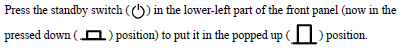
\includegraphics[width=\textwidth]{graphics/Agilent2011.png}
	\caption{Example of \UnicodeIEC{\symbol{"23FB}} usage in running text from 2011,
		in the installation guide for a network analyser.
		From \cite[Chapter 2, p.~24]{Agilent2011}.}
	\label{figure:example-of-use-Agilent} % label must come after caption
\end{figure}

\begin{figure}[h!]
	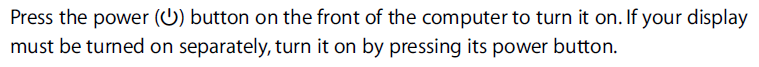
\includegraphics[width=\textwidth]{graphics/Apple2007.png}
	\caption{Example of \UnicodeIEC{\symbol{"23FB}} usage in running text from 2007,
		in the user's guide for a computer. From \cite[Chapter 1, p.~12]{Apple2007}.}
	\label{figure:example-of-use-Apple} % label must come after caption
\end{figure}

\begin{figure}[h!]
	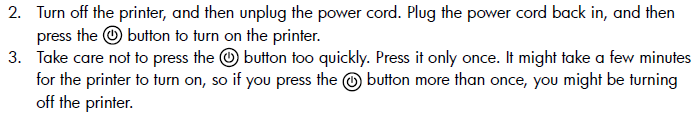
\includegraphics[width=\textwidth]{graphics/HP2009.png}
	\caption{Example of \UnicodeIEC{\symbol{"23FB}} usage in running text from 2009,
		in the setup guide for a printer. From \cite[p.~2]{HP2009}.}
	\label{figure:example-of-use-HP} % label must come after caption
\end{figure}

\begin{figure}[ht]
	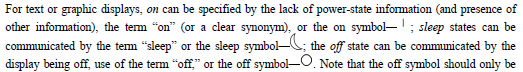
\includegraphics[width=\textwidth]{graphics/IEEE1621.png}
	\caption{Example of \UnicodeIEC{\symbol{"23FD}}, \UnicodeIEC{\symbol{"1F32D}},
		and \UnicodeIEC{\symbol{"2B58}} usage in running text from 2004,
		in a standards document. From \cite[\S 4.5.2, p.~7]{IEEE1621}.}
	\label{figure:example-of-use-IEEE} % label must come after caption
\end{figure}

\begin{figure}[ht]
	\centering
	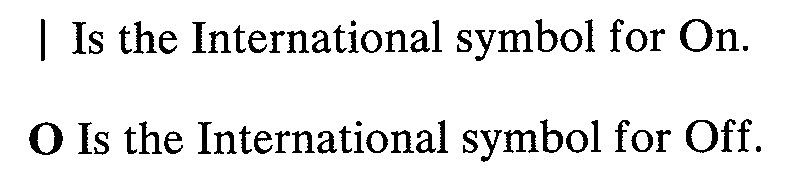
\includegraphics[width=0.5\textwidth]{graphics/IBM1984.png}
	\caption{Example of \UnicodeIEC{\symbol{"23FD}} and \UnicodeIEC{\symbol{"2B58}}
		usage in running text from 1984, in the user manual for a computer. From
		\cite[p.~1-11]{IBM1984}.}
	\label{figure:example-of-use-IBM} % label must come after caption
\end{figure}

\begin{figure}[ht]
	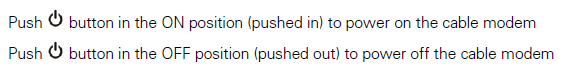
\includegraphics[width=\textwidth]{graphics/Motorola2010.png}
	\caption{Example of \UnicodeIEC{\symbol{"23FB}} usage in running text from 2010,
		in the installation guide for a cable modem. From \cite[p.~7]{Motorola2010}.}
	\label{figure:example-of-use-Motorola} % label must come after caption
\end{figure}

\begin{figure}[ht]
	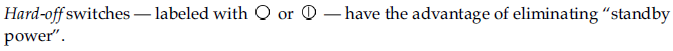
\includegraphics[width=\textwidth]{graphics/Nordman2002-0T.png}
	\caption{Example of \UnicodeIEC{\symbol{"2B58}} and \UnicodeIEC{\symbol{"23FC}}
		used in running text, in a monograph from 2002. From \cite[p.~4]{Nordman2002}
		(used by permission).}
	\label{figure:example-of-use-Nordman-0T} % label must come after caption
\end{figure}

\begin{figure}[ht]
	\centering
	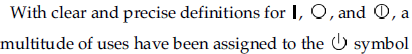
\includegraphics[width=0.8\textwidth]{graphics/Nordman2002-01TP.png}
	\caption{Example of \UnicodeIEC{\symbol{"23FD}}, \UnicodeIEC{\symbol{"2B58}},
		\UnicodeIEC{\symbol{"23FC}}, and \UnicodeIEC{\symbol{"23FB}} usage in running
		text, in a monograph from 2002. From \cite[p.~2]{Nordman2002} (used by permission).}
	\label{figure:example-of-use-Nordman-01TP} % label must come after caption
\end{figure}

\begin{figure}[ht]
	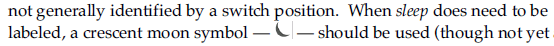
\includegraphics[width=\textwidth]{graphics/Nordman2002-S.png}
	\caption{Example of \UnicodeIEC{\symbol{"1F32D}} used in running text, in a
		monograph from 2002. From \cite[p.~2]{Nordman2002} (used by permission).}
	\label{figure:example-of-use-Nordman-S} % label must come after caption
\end{figure}

\begin{figure}[ht]
	\centering
	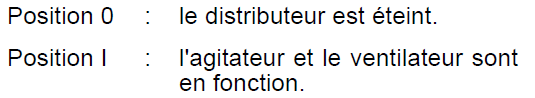
\includegraphics[width=0.8\textwidth]{graphics/Ugolini2013.png}
	\caption{Example of \UnicodeIEC{\symbol{"2B58}} and \UnicodeIEC{\symbol{"23FD}}
		used in running text from 2013, in the operator's manual for a coffee maker.
		From \cite[p.~18]{Ugolini2013}.}
	\label{figure:example-of-use-Ugolini} % label must come after caption
\end{figure}

\section{Character Properties}

Suggested character properties for the proposed symbols are given in Tables
\ref{table:character-properties-P}--\ref{table:character-properties-T} and
here in Unicode Character Database (UCD) format. The names are generally
similar to the names in IEEE 1621-2004.  None of the proposed names appear
already in the Character Name Index.

\begin{quote}
\begin{verbatim}
23FB;POWER SYMBOL;So;0;ON;;;;;N;;;;;
23FC;POWER ON-OFF SYMBOL;So;0;ON;;;;;N;;;;;
23FD;POWER ON SYMBOL;So;0;ON;;;;;N;;;;;
1F32D;BLACK WANING CRESCENT MOON;So;0;ON;;;;;N;;;;;
\end{verbatim}
\end{quote}

\begin{table}[htbp]
	\centering
	\begin{tabular}{ll}
		\textbf{Property} & \textbf{Suggested Value} \\
		\hline \\
		Code point                & 23FB \\
		Name                      & POWER SYMBOL \\
		General Category          & So \\
		Canonical Combining Class & 0 \\
		Bidirectional Class       & ON \\
		Decomposition Type/Decomposition Mapping \\
		Numeric Type \\
		Numeric Value \\
		Bidi Mirrored             & N \\
		Unicode 1 Name \\
		ISO Comment \\
		Simple Uppercase Mapping \\
		Simple Lowercase Mapping \\
		Simple Titlecase Mapping \\
    \end{tabular}
    \caption{Suggested character properties for \UnicodeIEC{\symbol{"23FB}}. This
		symbol is cross referenced to \UnicodeIEC{\symbol{"2B58}}.}
    \label{table:character-properties-P} % label must come after caption!
\end{table}

\begin{table}[htbp]
	\centering
	\begin{tabular}{ll}
		\textbf{Property} & \textbf{Suggested Value} \\
		\hline \\
		Code point                & 2B58 \\
		Name                      & HEAVY CIRCLE \\
		General Category          & So \\
		Canonical Combining Class & 0 \\
		Bidirectional Class       & ON \\
		Decomposition Type/Decomposition Mapping \\
		Numeric Type \\
		Numeric Value \\
		Bidi Mirrored             & N \\
		Unicode 1 Name \\
		ISO Comment \\
		Simple Uppercase Mapping \\
		Simple Lowercase Mapping \\
		Simple Titlecase Mapping \\
    \end{tabular}
    \caption{Suggested character properties for \UnicodeIEC{\symbol{"2B58}}. This
		symbol was unified in UTC \#138 with the alias POWER OFF SYMBOL and cross
		referenced to \UnicodeIEC{\symbol{"23FB}}.}
    \label{table:character-properties-0} % label must come after caption!
\end{table}

\begin{table}[htbp]
	\centering
	\begin{tabular}{ll}
		\textbf{Property} & \textbf{Suggested Value} \\
		\hline \\
		Code point                & 1F32D \\
		Name                      & BLACK WANING \\
		                          & CRESCENT MOON \\
		General Category          & So \\
		Canonical Combining Class & 0 \\
		Bidirectional Class       & ON \\
		Decomposition Type/Decomposition Mapping \\
		Numeric Type \\
		Numeric Value \\
		Bidi Mirrored             & N \\
		Unicode 1 Name \\
		ISO Comment \\
		Simple Uppercase Mapping \\
		Simple Lowercase Mapping \\
		Simple Titlecase Mapping \\
    \end{tabular}
    \caption{Suggested character properties for \UnicodeIEC{\symbol{"1F32D}}. This
		symbol is cross referenced to \UnicodeIEC{\symbol{"23FB}} and has the alias
		POWER SLEEP SYMBOL.}
    \label{table:character-properties-S} % label must come after caption!
\end{table}

\begin{table}[htbp]
	\centering
	\begin{tabular}{ll}
		\textbf{Property} & \textbf{Suggested Value} \\
		\hline \\
		Code point                & 23FD \\
		Name                      & POWER ON SYMBOL \\
		General Category          & So \\
		Canonical Combining Class & 0 \\
		Bidirectional Class       & ON \\
		Decomposition Type/Decomposition Mapping \\
		Numeric Type \\
		Numeric Value \\
		Bidi Mirrored             & N \\
		Unicode 1 Name \\
		ISO Comment \\
		Simple Uppercase Mapping \\
		Simple Lowercase Mapping \\
		Simple Titlecase Mapping \\
    \end{tabular}
    \caption{Suggested character properties for \UnicodeIEC{\symbol{"23FD}}.}
    \label{table:character-properties-1} % label must come after caption!
\end{table}

\begin{table}[htbp]
	\centering
	\begin{tabular}{ll}
		\textbf{Property} & \textbf{Suggested Value} \\
		\hline \\
		Code point                & 23FC \\
		Name                      & POWER ON-OFF \\
		                          & SYMBOL \\
		General Category          & So \\
		Canonical Combining Class & 0 \\
		Bidirectional Class       & ON \\
		Decomposition Type/Decomposition Mapping \\
		Numeric Type \\
		Numeric Value \\
		Bidi Mirrored             & N \\
		Unicode 1 Name \\
		ISO Comment \\
		Simple Uppercase Mapping \\
		Simple Lowercase Mapping \\
		Simple Titlecase Mapping \\
    \end{tabular}
    \caption{Suggested character properties for \UnicodeIEC{\symbol{"23FC}}.}
    \label{table:character-properties-T} % label must come after caption!
\end{table}

\subsection{Collation Order}\label{section:collation-order}

There is no required collation order, although there is an implied state transition
ordering:

\begin{quote}
Power states shall be understood to have physical relationships to each other.
Specifically, \emph{on} is taken to be above \emph{sleep}, and \emph{sleep} above
\emph{off}.
\end{quote}

\noindent \cite[\S 4.4, emphasis in original]{IEEE1621}. We suggest
\UnicodeIEC{\symbol{"23FB}}, \UnicodeIEC{\symbol{"2B58}},
\UnicodeIEC{\symbol{"1F32D}}, \UnicodeIEC{\symbol{"23FD}},
\UnicodeIEC{\symbol{"23FC}}. They exhibit no shaping behaviour and have
no particular required sorting order (except see the quoted paragraph
above). The characters are uncased. There is no special line-breaking
behaviour required. These characters are not meant for use in identifiers,
although they have been used for such.\footnote{This web site has a collection
of more than thirty examples of IEC 60417-5009 used in logo design:
\URL{http://www.logodesignlove.com/logos-using-the-standby-symbol}.} They are
stand-alone symbols.  They are not white-space characters and have no numeric
values. They are neither combining characters nor punctuation.

\section{The \emph{UnicodeIECsymbol} Font}

The five symbols included in the \emph{UnicodeIECsymbol} TrueType or OpenType font
are shown in Table~\ref{table:symbols}. Only these symbols exist in the font; if
an undefined character, for example `A' is called for in the font, the result is
implementation-defined.\footnote{In \hologo{XeTeX}, for example, the result of
`A' in \emph{UnicodeIECsymbol} is \UnicodeIEC{A}.  In OpenOffice Writer, the
result is the letter `A' but in a san-serif typeface.}

\begin{table}[htbp]
	\centering
	\begin{threeparttable}
		\begin{tabular}{clll}
			\textbf{Character} & \textbf{Applicable} & \textbf{How to} & \textbf{Unicode Name} \\
			& \textbf{Standard(s)} & \textbf{Type It} \\
			\hline \\
			\UnicodeIEC{\symbol{"23FB}}  & IEC 60417-5009 & \verb,&#x23FB;,  & POWER SYMBOL \\
			\UnicodeIEC{\symbol{"23FC}}  & IEC 60417-5010 & \verb,&#x23FC;,  & POWER ON-OFF SYMBOL \\
			\UnicodeIEC{\symbol{"23FD}}  & IEC 60417-5007 & \verb,&#x23FD;,  & POWER ON SYMBOL \\
			\UnicodeIEC{\symbol{"2B58}}  & IEC 60417-5008 & \verb,&#x2B58;,  & HEAVY \
			                                                                   CIRCLE\tnote{*} \\
			\UnicodeIEC{\symbol{"1F32D}} & IEEE 1621-2004 & \verb,&#x1F32D;, & BLACK WANING \\
										 &                &                  & CRESCENT \
																			   MOON\tnote{$\dagger$} \\
		\end{tabular}
		\begin{tablenotes}
			\item[*] {\footnotesize This character is aliased to POWER OFF SYMBOL.}
			\item[$\dagger$] {\footnotesize This character is aliased to POWER SLEEP SYMBOL.}
		\end{tablenotes}
	\end{threeparttable}
    \caption{All of the available glyphs in the \emph{UnicodeIECsymbol} font.}
    \label{table:symbols} % label must come after caption!
\end{table}

\begin{comment}
	Placement of symbols in the \emph{UnicodeIECsymbol} TrueType font was chosen
	thoughtfully so as to be mnemonic: `P' for power, `S' for sleep,
	`T' for toggling power on or off, and `1' and `0' for power-on and power-off,
	respectively; these mnemonics `fail gracefully' in text should the
	\emph{UnicodeIECsymbol} font happen to be unavailable.
\end{comment}

In text with normal spacing, the \UnicodeIEC{\symbol{"23FB}} characters
\UnicodeIEC{\symbol{"2B58}} look \UnicodeIEC{\symbol{"1F32D}} like
\UnicodeIEC{\symbol{"23FD}} this \UnicodeIEC{\symbol{"23FC}}.\footnote{The
spacing around \UnicodeIEC{\symbol{"23FD}} in the font appears wider because
the glyphs are fixed-width.}

\section{Anticipated Objections}

It might be argued that the meaning of \UnicodeIEC{\symbol{"23FB}} is
disputed between IEC 60417 and IEEE 1621-2004, {\it i.e.}, that IEC 60417
(as well as ISO 7000:2012) defined \UnicodeIEC{\symbol{"23FB}}
to mean `stand-by' and IEEE 1621-2004 changed it to mean `power'. We counter that
the issue is irrelevant to the Unicode Consortium for two reasons: firstly,
because the symbol itself is needed by writers, regardless of the fact that
`stand-by' has no consistent definition;\footnote{The term is routinely used to
mean \emph{off}, \emph{sleep}, \emph{on}, and other meanings that do not map
to a consistent power state at all.} and secondly, because IEEE 1621-2004 specifically
codifies existing practice; the number of devices using \UnicodeIEC{\symbol{"23FB}}
to mean `power' dwarfs the number of devices that use it to mean `stand-by'.
Furthermore,

\begin{quote}
No safety issue is introduced by the use of the symbol on a switch that causes
the device to go to a \emph{hard-off} state.
\end{quote}

\noindent \cite[\S 4.3, emphasis in original]{IEEE1621}.

There are, of course, many characters in Unicode already resembling circles
(\UnicodeIEC{\symbol{"2B58}}), or lines (\UnicodeIEC{\symbol{"23FD}}), or the
crescent moon (\UnicodeIEC{\symbol{"1F32D}}). None of the existing
characters, however, has anything semantically to do with the concepts of `power',
`switch', `toggle', or `interrupter'. There are several occurrences of the crescent
moon, but none showing the \UnicodeIEC{\symbol{"1F32D}} phase; IEEE 1621-2004 intended
the symbol to be different from other Unicode instances of a crescent moon. There
are eleven occurrences of the word `power' in Version 6.3.0 of the Unicode standard
(Table \ref{table:power}) but none has anything to do with device control
\cite{Unicode2013}.

\section{Drawing the Symbols}

The proposed characters are not part of any script and the precise form of
their drawing is not critical. As IEEE 1621-2004 says:

\begin{quote}
In accordance with IEC 80416-3, symbols can be filled, be rotated, have their lines
thickened, or be used on digital displays, as long as an ordinary user can recognize
the symbol correctly.
\end{quote}

\noindent \cite[\S 4.3]{IEEE1621}.

\begin{table}[htbp]
	\centering
	\begin{tabular}{lcl}
		\textbf{Section} & \textbf{Code Point} & \textbf{Description} \\
		\hline \\
		Telugu fractions \
			& 0C78 & TELUGU FRACTION DIGIT \\
		and weights	& & ZERO FOR ODD POWERS \\
				& & OF FOUR \\
			& 0C79 & TELUGU FRACTION DIGIT \\
				& & ONE FOR ODD POWERS \\
				& & OF FOUR \\
			& 0C7A & TELUGU FRACTION DIGIT \\
				& & TWO FOR ODD POWERS \\
				& & OF FOUR \\
			& 0C7B & TELUGU FRACTION DIGIT \\
				& & THREE FOR ODD POWERS \\
				& & OF FOUR \\
			& 0C7C & TELUGU FRACTION DIGIT \\
				& & ONE FOR EVEN POWERS \\
				& & OF FOUR \\
			& 0C7D & TELUGU FRACTION DIGIT \\
				& & TWO FOR EVEN POWERS \\
				& & OF FOUR \\
			& 0C7E & TELUGU FRACTION DIGIT \\
				& & THREE FOR EVEN \\
				& & POWERS OF FOUR \\
		\hline
		Miscellaneous \
			& 26EE & GEAR WITH HANDLES \\
		Symbols & & (= power plant, power \\
				& & substation) \\
		\hline
		Kangxi Radicals \
			& 2F12 & KANGXI RADICAL POWER \\
		\hline
		Yijing Hexagram Symbols \
			& 4DE1 & HEXAGRAM FOR GREAT \\
				& & POWER \\
		\hline
		Mathematical \
			& 1D4AB & MATHEMATICAL SCRIPT \\
		Alphanumeric Symbols & & CAPITAL P (= power set) \\
    \end{tabular}
    \caption{All occurrences of `power' in the Unicode Standard, Version 6.3.0.}
    \label{table:power} % label must come after caption!
\end{table}

\subsection{Severability}

Of all the characters in Table \ref{table:symbols}, the most needed is
\UnicodeIEC{\symbol{"23FB}}. We included the others in this proposal because
they form a logical group. If, however, there is any objection to inclusion of
\UnicodeIEC{\symbol{"23FD}}, \UnicodeIEC{\symbol{"2B58}}, \UnicodeIEC{\symbol{"23FC}},
or \UnicodeIEC{\symbol{"1F32D}}, the one we most need is \UnicodeIEC{\symbol{"23FB}}.

\section{Sponsors}

The address for correspondence is:

\begin{quote}
	Joe Loughry \\
	6214 South Krameria Street \\
	Centennial, CO 80111-4243 \\
	USA

	\medskip Tel.\ +1 303 221 4380

	\medskip Email:~\texttt{joe.loughry@stx.ox.ac.uk}
\end{quote}

\noindent The other sponsors' postal addresses are:

\begin{quote}
	Terence Eden \\
	24 Thames View Road \\
	Oxford, OX4 4TG \\
	ENGLAND

	\medskip Email: \texttt{terence.eden@shkspr.mobi}
\end{quote}

\noindent and

\begin{quote}
	Bruce Nordman \\
	90-2000 \\
	1 Cyclotron Road \\
	Lawrence Berkeley National Laboratory \\
	Berkeley, CA 94720-8130 \\
	USA

	\medskip Tel.\ 510-486-7089

	\medskip Email: \texttt{BNordman@LBL.gov}
\end{quote}

\section{Summary and Conclusion}

The \UnicodeIEC{\symbol{"23FB}}, \UnicodeIEC{\symbol{"2B58}},
\UnicodeIEC{\symbol{"1F32D}}, \UnicodeIEC{\symbol{"23FD}}, and
\UnicodeIEC{\symbol{"23FC}} symbols are needed by technical writers
to produce manuals in which these important symbols are searchable
in plain text. Because they were invented by the standards body to
be distinctive, new, and unambiguous, there is no confusion with existing
scripts. They have been in use in running text for at least thirty years.
The suggested character properties are straightforward. We provide along with this
proposal TrueType and OpenType fonts called \emph{UnicodeIECsymbol}
containing the new symbols; the fonts are made available with no restrictions.

\bibliographystyle{plain}
\bibliography{consolidated_bibtex_file}

\vfill
\noindent{\tiny This document was made with \hologo{XeTeX}. Build \input{build_counter.txt}}

\newpage
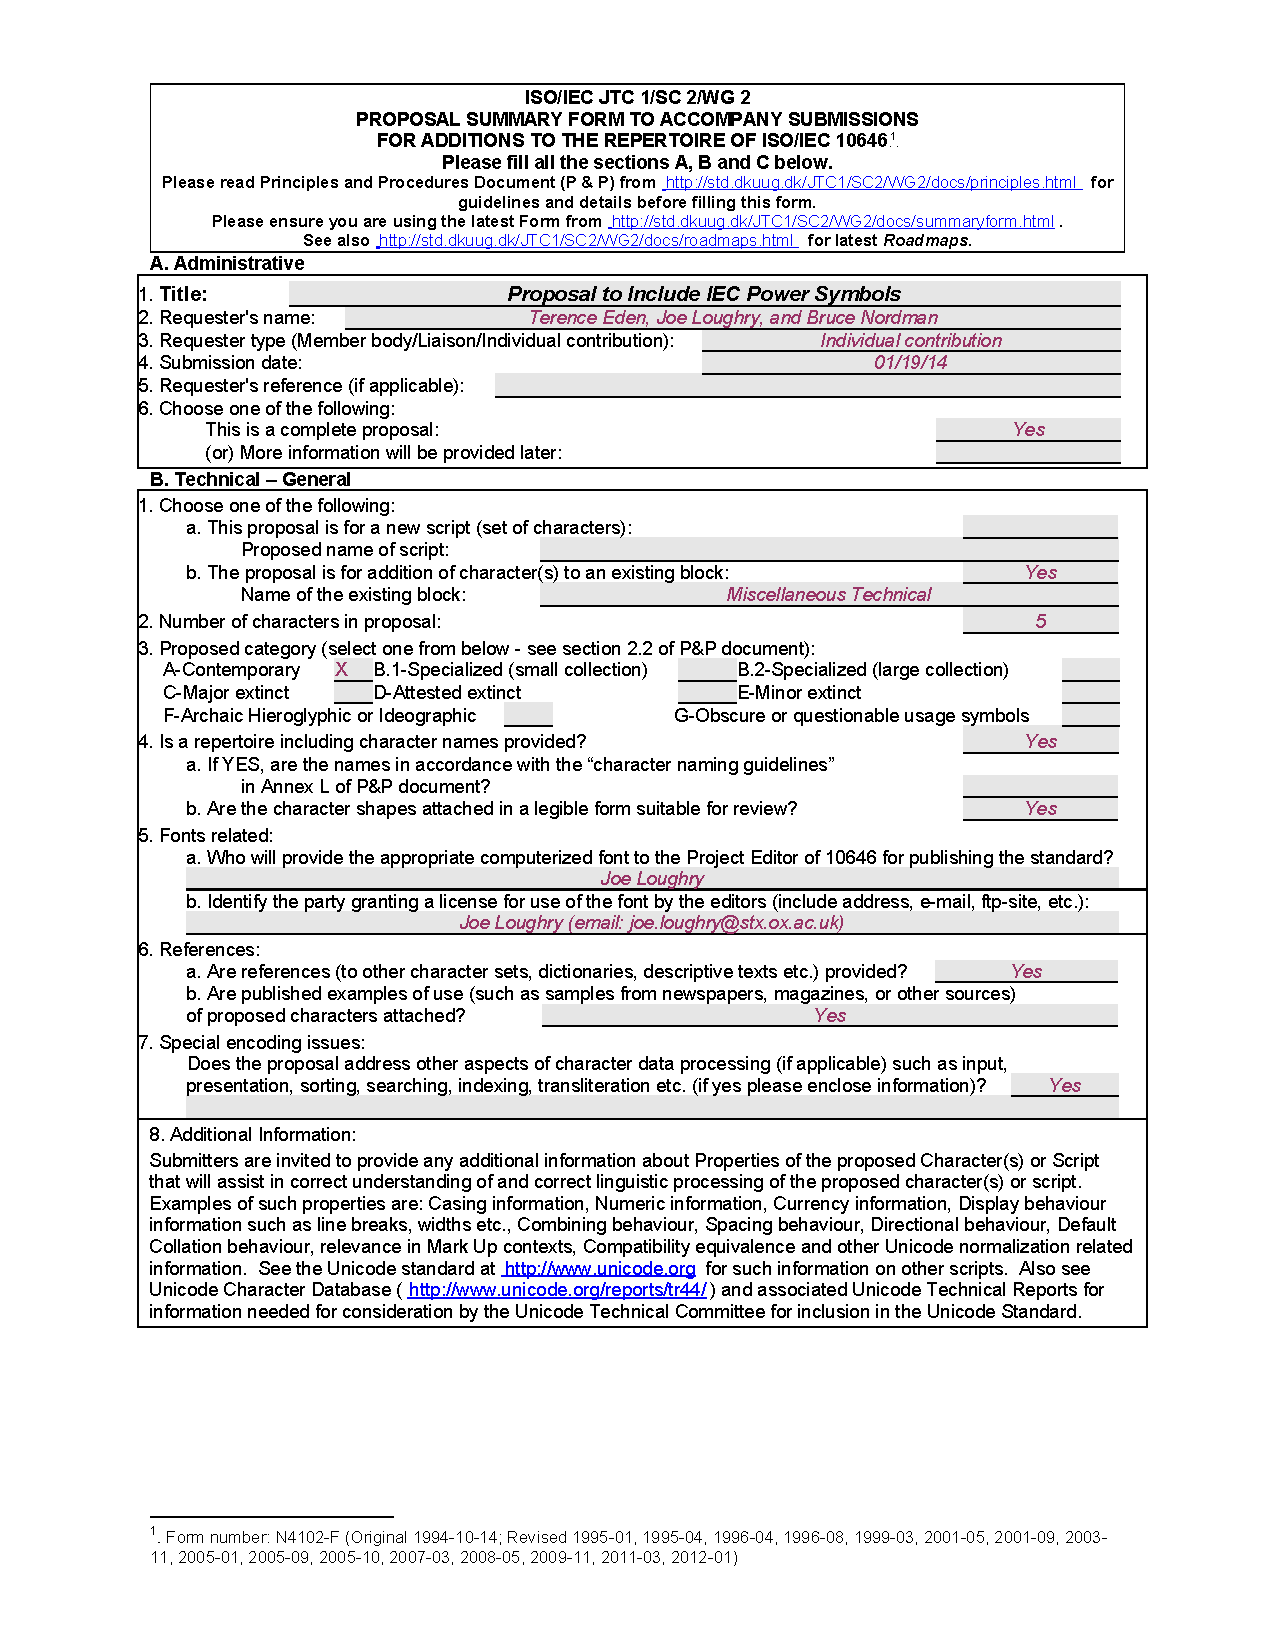
\includepdf[pages={1-2}]{ISO_submission_form/n4102-form-completed.pdf}

\end{document}

